\documentclass[sigconf]{acmart}

\usepackage{multirow}
\usepackage{graphicx}
\usepackage{subcaption}
\captionsetup{subrefformat=parens}
\usepackage[ruled, vlined]{algorithm2e}
% \usepackage{algorithm}
% \usepackage{algpseudocode}

\graphicspath{ {images/} }

\SetKwBlock{Interface}{Interface:}{}
\SetKwBlock{State}{State:}{}
\SetKwBlock{Requests}{Requests:}{}
\SetKwBlock{Indications}{Indications:}{}

\SetKwProg{UponTimer}{Upon Timer}{ do:}{}
\SetKwProg{Procedure}{Procedure}{ do:}{}
\SetKwProg{Upon}{Upon}{ do:}{}
\SetKwProg{If}{If}{ do:}{}
\SetKwProg{Foreach}{Foreach}{ do:}{}

\SetKwComment{Comment}{/* }{ */}
\SetKw{Trigger}{Trigger}
\SetKw{Call}{Call}
\SetKw{CancelTimer}{Cancel Timer}
\SetKw{SetupTimer}{Setup Timer}
\SetKw{SetupPeriodicTimer}{Setup Periodic Timer}

%%
%% \BibTeX command to typeset BibTeX logo in the docs
\AtBeginDocument{%
  \providecommand\BibTeX{{%
    \normalfont B\kern-0.5em{\scshape i\kern-0.25em b}\kern-0.8em\TeX}}}

%% Rights management information.  This information is sent to you
%% when you complete the rights form.  These commands have SAMPLE
%% values in them; it is your responsibility as an author to replace
%% the commands and values with those provided to you when you
%% complete the rights form.
\setcopyright{acmcopyright}
\copyrightyear{2022}
\acmYear{2022}
%\acmDOI{10.1145/1122445.1122456}

%% These commands are for a PROCEEDINGS abstract or paper.
\acmConference[ASD22/23]{The first project delivery of ASD2223}{2022}{Faculdade de Ciências e Tecnologia, NOVA University of Lisbon, Portugal}
\acmBooktitle{The Projects of ASD - first delivery, 2021, Faculdade de Ciências e Tecnologia, NOVA University of Lisbon, Portugal}
%\acmPrice{15.00}
%\acmISBN{978-1-4503-XXXX-X/18/06}


%%
%% Submission ID.
%% Use this when submitting an article to a sponsored event. You'll
%% receive a unique submission ID from the organizers
%% of the event, and this ID should be used as the parameter to this command.
%%\acmSubmissionID{123-A56-BU3}

%%
%% The majority of ACM publications use numbered citations and
%% references.  The command \citestyle{authoryear} switches to the
%% "author year" style.
%%
%% If you are preparing content for an event
%% sponsored by ACM SIGGRAPH, you must use the "author year" style of
%% citations and references.
%% Uncommenting
%% the next command will enable that style.
%%\citestyle{acmauthoryear}

%%
%% end of the preamble, start of the body of the document source.
\begin{document}

%%
%% The "title" command has an optional parameter,
%% allowing the author to define a "short title" to be used in page headers.
\title{Strongly Consistent Replicated HashMap}

%%
%% The "author" command and its associated commands are used to define
%% the authors and their affiliations.
%% Of note is the shared affiliation of the first two authors, and the
%% "authornote" and "authornotemark" commands
%% used to denote shared contribution to the research.
\author{António Duarte}
\authornote{Student number 58278. %responsibility?
}
\email{an.duarte@campus.fct.unl.pt}
\affiliation{%
    \institution{MIEI, DI, FCT, UNL}
}

\author{Diogo Almeida}
\authornote{Student number 58369. %responsibility?
}
\email{daro.almeida@campus.fct.unl.pt}
\affiliation{%
    \institution{MIEI, DI, FCT, UNL}
}

\author{Diogo Fona}
\authornote{Student number 57940. %responsibility?
}
\email{d.fona@campus.fct.unl.pt}
\affiliation{%
    \institution{MIEI, DI, FCT, UNL}
}

%%
%% By default, the full list of authors will be used in the page
%% headers. Often, this list is too long, and will overlap
%% other information printed in the page headers. This command allows
%% the author to define a more concise list
%% of authors' names for this purpose.
\renewcommand{\shortauthors}{Duarte, Almeida, and Fona.}

%%
%% The abstract is a short summary of the work to be presented in the
%% article.
\begin{abstract}
Strong consistency in replicated hash maps refers to the property of the data being kept in sync across all of the replicas in the system. This means that, at any given time, all of the replicas will have the same set of key-value pairs, and any changes made to the data on one replica will be immediately reflected on all of the other replicas.

Agreement protocols like Paxos are used to ensure that the replicas in a distributed system can come to consensus on the state of the data, even in the presence of failures. This is important for maintaining strong consistency in replicated hash maps, as it ensures that the replicas are all in agreement on the state of the data and can continue to operate correctly.

In this work we propose a replicated hash map which uses an agreement protocol to maintain strong consistency between the replicas of the system. We further conduct an experimental evaluation where the system is tested with increasing loads of operation requests by clients. 

\end{abstract}

%% This command processes the author and affiliation and title
%% information and builds the first part of the formatted document.
\maketitle

\section{Introduction}

A replicated hash map is a distributed data structure that allows for efficient access to data across a network of machines. It uses the concept of a hash map, which is a data structure that stores key-value pairs and allows for efficient lookup of values based on their associated keys. In a replicated hash map, multiple copies of the hash map are maintained on different machines in the network, and agreement protocols can be used to ensure that all copies are kept consistent with each other.

Paxos \cite{leslie1998part} \cite{lamport2001paxos} \cite{van2015paxos} and Multi-Paxos \cite{lamport2001paxos} \cite{du2009multi} \cite{van2015paxos} are examples of agreement protocols that are commonly used in distributed systems to achieve consistency in replicated data structures. The Paxos algorithm is a method for reaching consensus among a group of nodes in a distributed system. Multi-Paxos is a variant of the Paxos algorithm that improves performance in in scenarios where there are multiple replicated data structures, or multiple instances of the Paxos algorithm running concurrently.

In both Paxos and Multi-Paxos, nodes in the distributed system communicate with each other using a series of rounds, during which they propose values, "vote" on the proposed values, and ultimately agree on a single value to be chosen. Once consensus has been reached, the agreed-upon value can be safely used by the nodes in the system, ensuring that all copies of the replicated data are consistent with each other.

Operations decided with agreement have to be executed in the same order in every replica so they don't diverge their state. State machine replication is a technique used in distributed systems to ensure that the same sequence of operations is performed on all replicas of a given state machine. This is typically achieved through the use of an agreement protocol, which is used to coordinate the actions of the replicas and reach consensus on the order in which operations should be applied.

In this work, we present a proposal for a replicated hash map application that makes use of an agreement protocol, either Paxos or Multi-Paxos, and state machine replication implemented with the Babel \cite{fouto2022babel} Java framework.

The remainder of this article is organized as follows: In Section 2 we will be going over the Related Work, explaining more thoroughly the mentioned protocols; In Section 3 we will go over the details of our implementation of the protocols and how they interact with each other; In Section 4 we present the results of our experimental evaluation, testing the system with an increasing throughput of clients issuing operations. In Section 5 we will summarize and take conclusions on this work.


\section{Related Work}

\subsection{Consensus}

The consensus problem in a distributed system refers to the challenge of achieving agreement among a group of processes or nodes, on a single data value. This problem is crucial in distributed systems, as it allows a network of nodes to reach a consistent state. A correct consensus protocol must uphold the following properties:

\begin{itemize}
    \item \textbf{Termination} Every correct process eventually decides a value.
    \item \textbf{Validity} If a process decides on a value \textit{v}, then \textit{v} was proposed by some process.
    \item \textbf{Integrity} No process decides twice.
    \item \textbf{Uniform Agreement} No two processes decide differently. 
\end{itemize}

Consensus, as specified in it's formal definition, has been proven to be impossible under an asynchronous system with the crash-fault model \cite{fischer1985impossibility}, it is, although, possible to achieve a practically useful version by relaxing one or some of its properties.

\subsubsection{Paxos} 

Paxos is a distributed agreement protocol that achieves a weaker version of consensus by relaxing the \textbf{Termination} property. This ensures that the system only progresses if it behaves in a synchronous way for a long enough period.

In Paxos, for ease of understanding, each replica is often subdivided into three different roles, each with different responsibilities:

\begin{itemize}
    \item \textbf{Proposers}, responsible for proposing new values for the system to decide on.
    \item \textbf{Acceptors}, they promise on proposed values, and lock-in values by accepting them.
    \item \textbf{Learners}, the role responsible for understanding that a value has been decided on. 
\end{itemize}

There are two main phases in the Paxos protocol: the prepare phase and the accept phase. In the prepare phase, the proposers send prepare requests asking all the acceptors to promise not to accept any other proposals. After receiving a majority quorum of promises, in the accept phase proposers send their proposed values to the acceptors. After this, the learners will become aware of the decided value. This can be achieved in a variety of ways, for example, the acceptors send the accepted values to all learners.

One of the key benefits of Paxos is that it is able to tolerate failures. For example, if a replica fails during the prepare phase its prepare will be overwritten by a future one, and if a replica fails during the accept phase the other replicas can still come to agreement on the value without it, as it requires a majority quorum to decide. This makes Paxos a robust and fault-tolerant protocol for achieving consensus in distributed systems.

The main disadvantage of using Paxos in opposition to some of its alternatives, is that for each value that we're deciding on, we need to use a new instance of the protocol. This implies that everytime we want to make a decision, we need to redo all the phases of the algorithm, including the prepare phase, which impacts the performance of the protocol, due to the added round trips in the protocol's communication steps. 

\subsubsection{Multi-Paxos}

% Multi-Paxos is a variant of the Paxos protocol that is used when there are multiple replicas that need to agree on multiple values. This can be useful in situations where there are multiple sources of data that need to be kept in sync across the replicas.

Multi-Paxos is a variant of the Paxos protocol and as such, it also uses two phases in which the replicas communicate with each other to come to agreement on values. The distinction here is a distinguished proposer is selected (also referred to as leader) to be the only one proposing values.

Additionally, in contrary to Paxos, there is only a single instance of the protocol which contains the shared state for decisions made for multiple values, which most importantly contains the distinguished proposer.

The benefit of using a distinguished proposer is that it relinquishes the need of the prepare phase when making multiple decisions. This means only accept messages are sent by the leader which removes one round-trip-time from the process of making a decision.

The leader is elected by using a prepare phase, either when first initializing the system, or when a participating replica suspects that the current leader has crashed.


\section{Implementation}

The system is divided in three layers: 1. the application that holds the hash map functionality. The app sends operations to 2. the state machine so they are ordered with operations from other replicas and the state is kept consistent. In turn, the state machine issues operations to 3. an agreement protocol, which proposes them and eventually agrees between the replicas on which are executed in each instance.

We implemented the replicated hash map application, the state machine replication protocol, Paxos and Multi-Paxos using the Babel Java framework, ensuring both agreement protocols are compared fairly.

\subsection{Application}

The replicated hash map application layer receives requests from clients to perform operations based on its functionality. These operations are equivalent to the ones performed on a local hash map: \texttt{Get(Key)} and \texttt{Put(Key, Value)}. 

For each request a unique number is assigned which is associated to the client so it knows who to reply to later. The request is sent to the state machine replication to order it. Later that request's outcome is delivered to the application where the state is changed and a response to that operation is delivered to the client.

\subsection{State Machine Replication}

Upon receiving an order request, the state machine will either buffer it if the replica did not join the system yet or propose it to the agreement protocol where it will eventually be ordered.

After an operation decision from the agreement protocol, the state machine will send it to the application if it is in order. If not, it will hold it until it gets all the operations that precede it. 

\subsubsection{Operation Batching}

An optimization we implemented is operation batching. Batches are a list of operations the state machine receives from the application. A batch is formed from operations received in a time span, or until it contains enough operations. 

Thanks to this, the state machine will issue a request to the agreement protocol for each batch instead of for each single operation. When a batch is returned from agreement and then is the next in order to be executed, every operation in it will be delivered individually to the application.

This optimization greatly increases performance as the execution of the agreement is the step that leverages more execution time, more so with a bigger amount of replicas.

\subsubsection{Membership Changes}

% Explain how membership changes are handles and executed with agreement

The state machine can handle membership changes by using special commands, which are not originated from the application, that add and remove members. To add or remove a member one of these is issued to the agreement protocol. The membership change takes place when the commands are eventually executed.

In the case of a new replica wanting to join the system, it contacts a replica that is already in it and request it to join. In turn, the one receving the request issues the command to add a new member to the agreement protocol and when it later executes that command it sends the joining replica the information it requires, the current instance in the agreement protocol, the membership and the application state at that instance.

In the case of a replica detecting that another is down, it issues the command to remove a member to the the agreement protocol. After it is executed, the replica in question is removed from every replica's membership set. If many replicas simultaneously detect that one has failed  they will all issue the remove member command, but that is not an issue because the membership will end up having the same state.  

We note that these special commands are not batched, only operations that come from the application are. 

\subsubsection{Handling Leadership}

When using agreement protocols that have the notion of a leader such as Multi-Paxos, one of the replicas is considered the leader. The leader is responsible for ordering all the operations and so the other replicas will forward their operations to the leader instead of issuing them directly to the agreement protocol. Because of this, the state machine needs to know who is the leader, besides the agreement protocol.

A replica will attempt to take leadership in the following circumstances:
\begin{enumerate}
\item There is no leader and the replica has an operation it needs to order. This happens in the beggining of the system.
\item The leader is suspected to be unreachable, whether it crashed or lost connection.
\item The replica has lost some operations and is unable to execute the new ones because they depend on the lost ones. The replica only considers operations to be lost if it is missing them for a certain amount of time.
\end{enumerate}

In the case of Multi-Paxos, in each replica it will notify its state machine about a new leader when it accepts a prepare request from another replica. When a leader change is detected, a replica will send all its pending operations to the new leader.

\subsection{Agreement}

The agreement protocols, Paxos and Multi-Paxos, were implemented as indicated in their specifications. They can be interchanged easily using the same implemented state machine.


\section{Experimental Evaluation}

\subsection{Setup}

\begin{table}[h]
    \centering
    \caption{Protocol Parameters}
    \label{tab:parameters}
    \resizebox{\columnwidth}{!}{%
    \begin{tabular}{|l|l|r|}
    \hline
    \textbf{Protocol}              & \textbf{Parameter}  & \textbf{Value} \\ \hline
    \multirow{2}{*}{Clients}       & \% Reads            & 50\%           \\
                                   & \% Writes           & 50\%           \\ \hline
    \multirow{4}{*}{State Machine} & Leader Timeout      & 3s             \\
                                   & Batch Build Timeout & 5ms            \\
                                   & Batch Max Size      & 64             \\
                                   & Command Timeout     & 1s             \\ \hline
    Agreement                      & Proposal Timeout    & 200ms          \\ \hline
    \end{tabular}%
    }
\end{table}

The static configuration of each protocol and clients used in this experimental evaluation are presented in Table~\ref{tab:parameters}.

\textbf{Testbench:} the evaluation was conducted using a docker setup with a container per replica and a container for all the YCSB clients, using two machines with a 2x Intel Xeon Gold 6346 CPU, 128 GiB of DDR4 3200MHz RAM, and 1 Gbps of network bandwidth. One of the machines contained the clients and the other the replicas.

\subsection{Results}

\begin{figure}[htp]
    
\begin{subfigure}{\linewidth}
    \centering
    \caption{128 byte operations}
    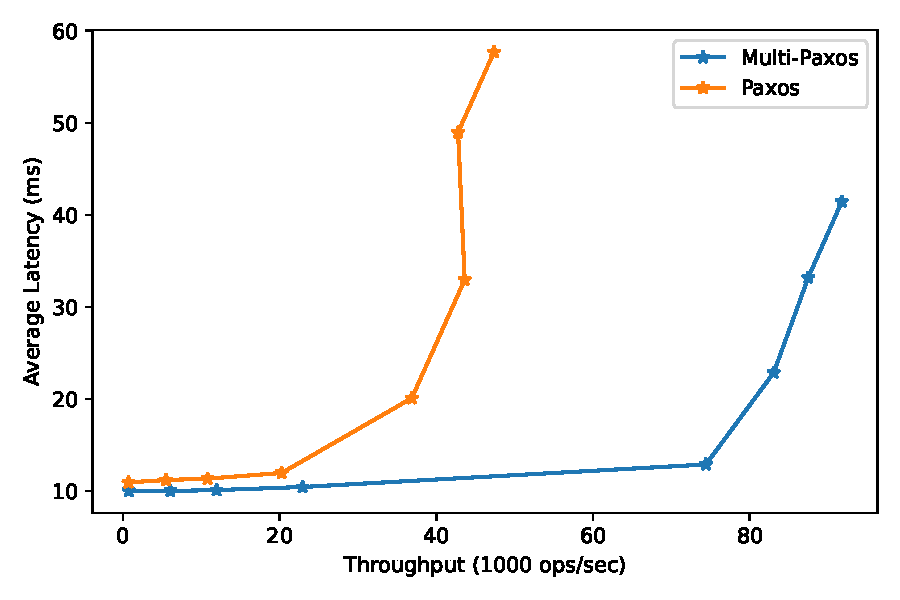
\includegraphics[width=\textwidth]{3R_128B.pdf}
    \label{fig:3replicas-128}
\end{subfigure}

\begin{subfigure}{\linewidth}
    \centering
    \caption{1024 byte operations}
    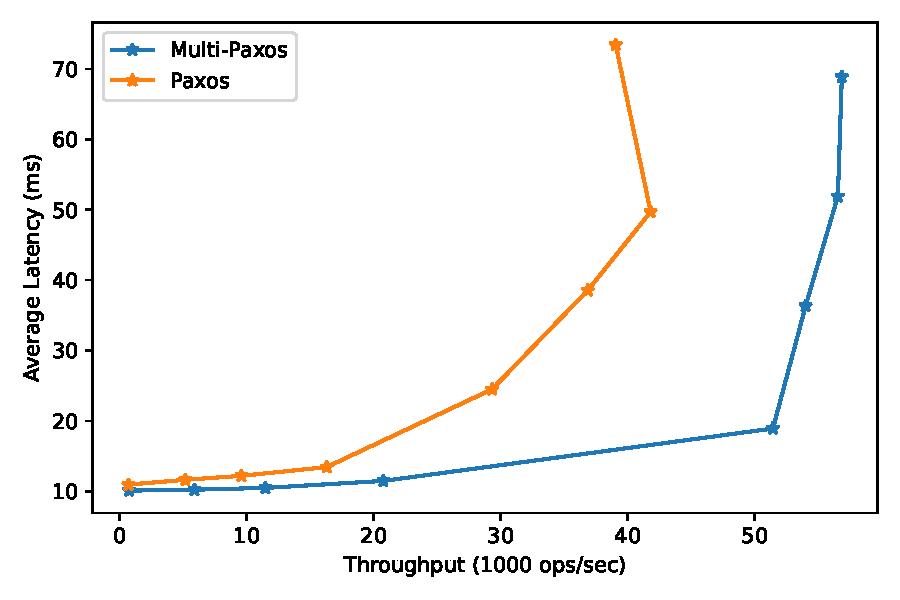
\includegraphics[width=\textwidth]{3R_1024B.pdf}
    \label{fig:3replicas-1024}
\end{subfigure}

\caption{Performance for operations over 3 replicas.}
\label{fig:3replicas}

\end{figure}

\begin{figure}[htp]
    
\begin{subfigure}{\linewidth}
    \centering
    \caption{128 byte operations}
    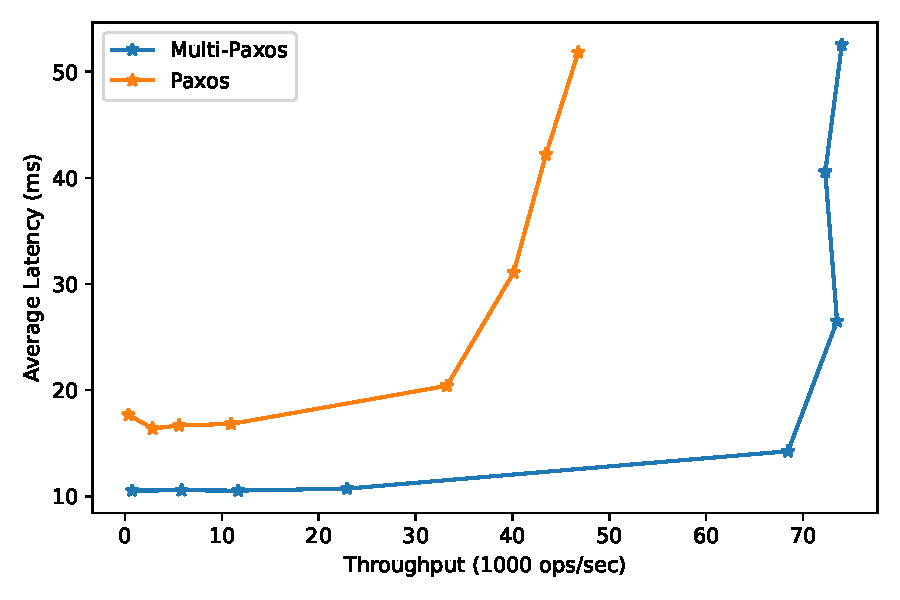
\includegraphics[width=\textwidth]{6R_128B.pdf}
    \label{fig:6replicas-128}
\end{subfigure}

\begin{subfigure}{\linewidth}
    \centering
    \caption{1024 byte operations}
    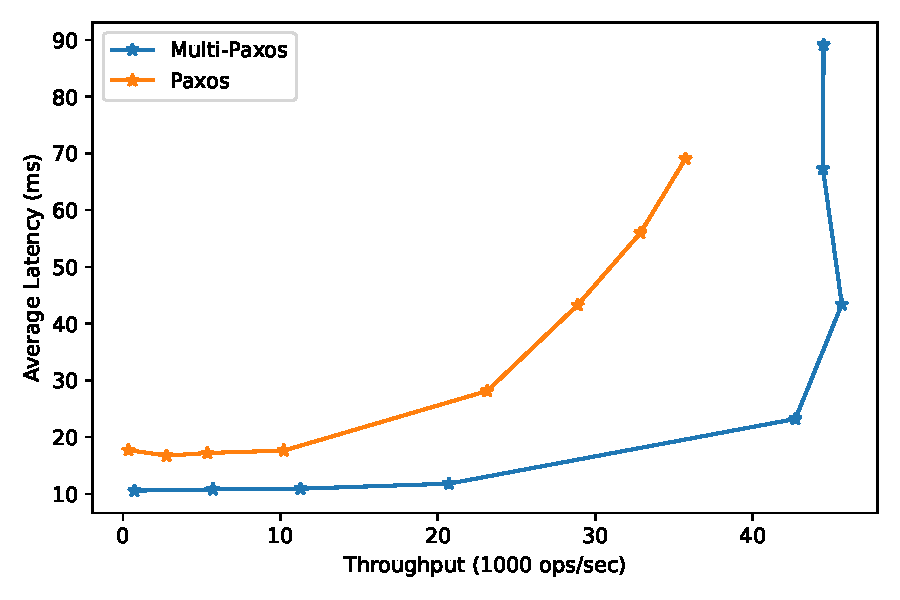
\includegraphics[width=\textwidth]{6R_1024B.pdf}
    \label{fig:6replicas-1024}
\end{subfigure}

\caption{Performance for operations over 6 replicas.}
\label{fig:6replicas}

\end{figure}

Figures~\ref{fig:3replicas} and~\ref{fig:6replicas} present throughput-latency plots of the system with both agreement protocols, different amount of replicas and different operation payload sizes. 

In all of the figures we can see that Multi-Paxos outperforms Paxos, saturating at a much higher throughput. This is expected since using a distinguished proposer, Multi-Paxos avoids the contention that Paxos suffers from when there are multiple proposers trying to propose a value at the same time.

Even when both don't show saturation, we can observe Multi-Paxos still outperforms Paxos by a fixed latency amount with six replicas. Possible reasons for this are:
\begin{enumerate}
    \item In Multi-Paxos the leader only requires one RTT to propose a command. Since each replica should handle one sixth of the clients and the leader can respond faster to clients, then it should be responsible for more than one sixth of the total operations during the test run causing the average response latency to be lower.
    \item The total amount of messages and payload sent between replicas is lower in Multi-Paxos, this means less CPU time is spent on message passing and processing which in turn can improve latency. This happens because, even though non-leader replicas require two RTTs to propose a command, they only need to forward the command to the leader instead of sending multiple prepare requests to all acceptors and have those acceptors send back responses.
\end{enumerate}

\section{Conclusions}

We evaluated the performance of a replicated hashmap system using state-machine replication with two different agreement protocols we implemented: Paxos and Multi-Paxos.

Our experimental results demonstrate that Multi-Paxos has a superior performance over Paxos in this context. Multi-Paxos was able to achieve a higher success rate in committing updates to the hashmap, with lower overall latency and fewer retries due to its use of a leader. This results in Multi-Paxos handling a much bigger amount of operation throughput than Paxos.

Overall, these findings suggest that Multi-Paxos is a valuable alternative to Paxos in replicated hash map systems, and further research into its use in other distributed systems contexts is warranted.

%%
%% The acknowledgments section is defined using the "acks" environment
%% (and NOT an unnumbered section). This ensures the proper
%% identification of the section in the article metadata, and the
%% consistent spelling of the heading.
\begin{acks}
    To João Leitão, for teaching us how to implement protocols and write good reports.
\end{acks}

%%
%% The next two lines define the bibliography style to be used, and
%% the bibliography file.
\bibliographystyle{ACM-Reference-Format}
\bibliography{acmart}

\end{document}
\endinput
%%
%% End of file `sample-sigconf.tex'